\section{Progress}

\begin{frame}{Overall Design}
    \begin{figure}[!htb]
        \centering
        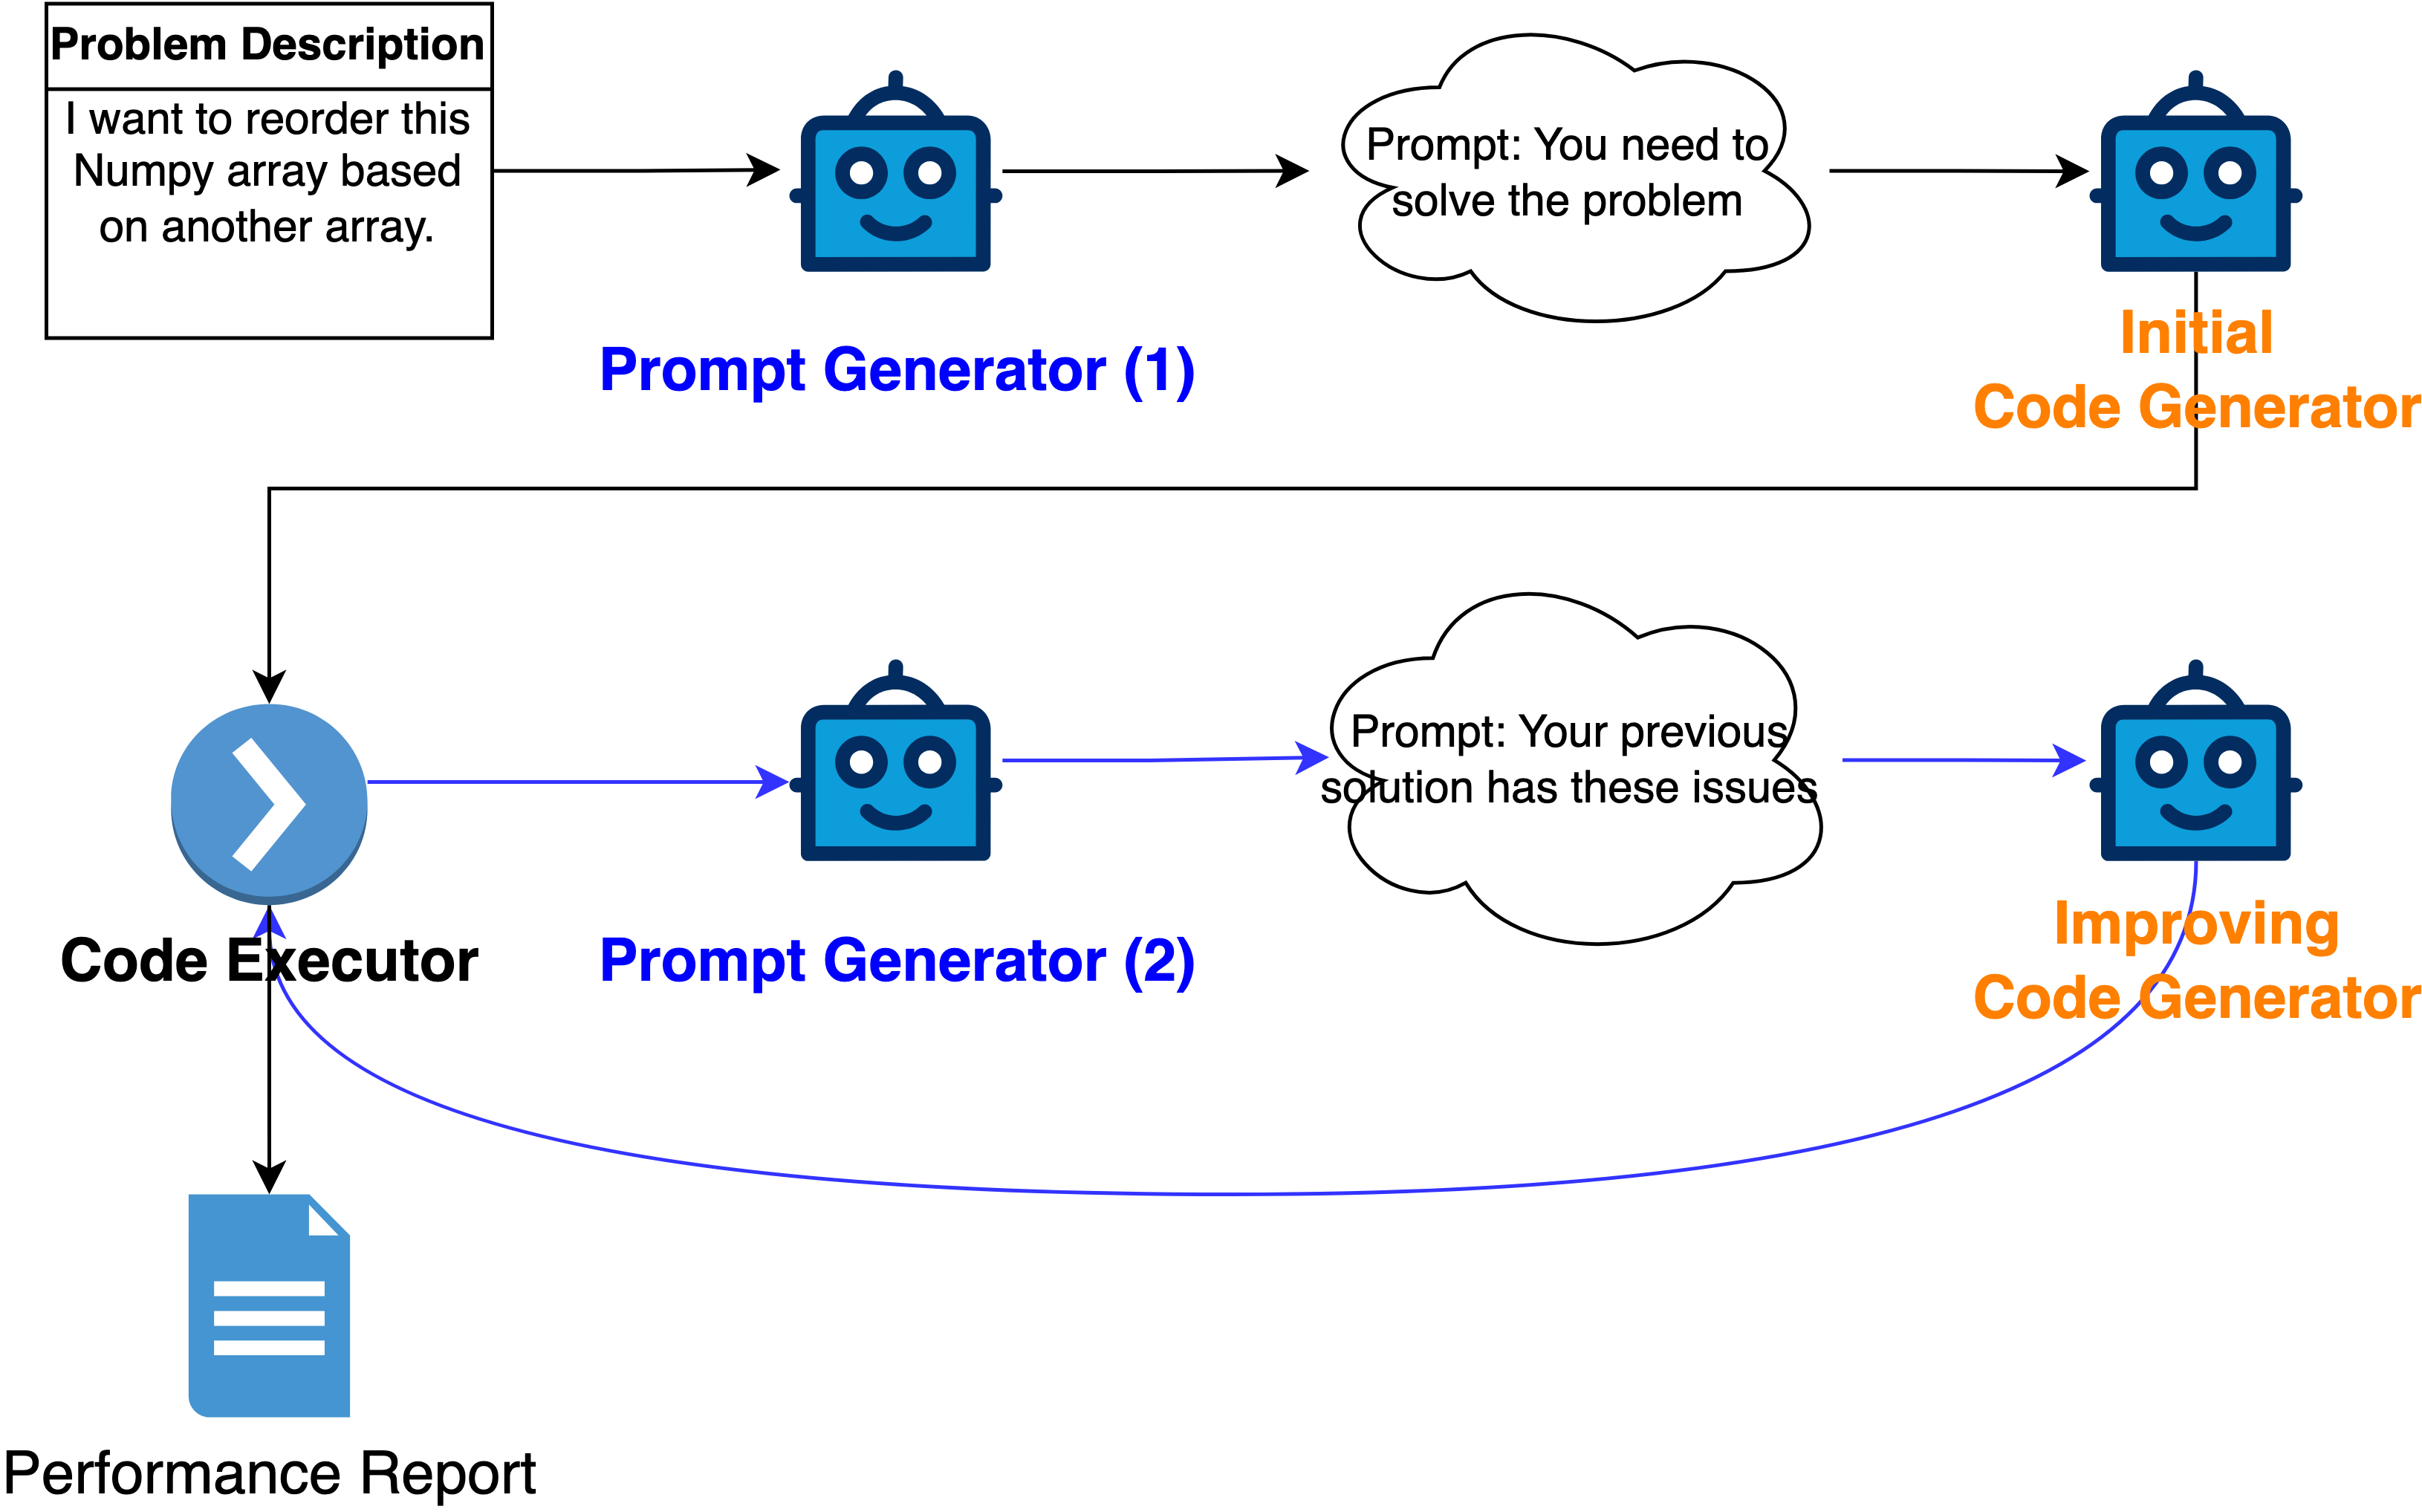
\includegraphics[width=0.9\textwidth]{img/selfdebug_design}
        \captionsetup{font=small,labelformat=empty}
        \caption{The modules of the proposed system.}
    \end{figure}
\end{frame}

\begin{frame}{Progress Update \: 08 Mar 2024}
    Completed:
    \begin{itemize}
        \item Prompt Generator (1) with Zero-shot prompts (baseline)
        \item Initial Code Generator with ChatGPT 3.5 API
        \item Code Executor on Virtual environment to run test cases
        \item Performance Report using accuracy score
    \end{itemize}

    Baseline Results:
    \begin{tabular}{lr}
        Library    & Accuracy \\
        \hline
        Matplotlib & 18.06\%  \\
        Scipy      & 16.04\%  \\
        Pandas     & 8.93\%   \\
        Numpy      & 5.91\%   \\
        Sklearn    & 9.57\%   \\
        Tensorflow & 17.78\%  \\
        Pytorch    & 2.94\%   \\
    \end{tabular}
\end{frame}

\begin{frame}{Progress Update \: 08 Mar 2024}
    Next Steps:
    \begin{itemize}
        \item Prompt Generator (2) with CoT prompts based on code execution feedback
        \item Improving Code Generator
    \end{itemize}
\end{frame}

\begin{frame}{Progress Update \: 25 Mar 2024}
    Completed:
    \begin{itemize}
        \item Prompt Generator (1) with CoT prompts
    \end{itemize}

    Baseline Results:
    \begin{tabular}{lr}
        Library    & Accuracy \\
        \hline
        Matplotlib & 31.61\%  \\
        Scipy      & 12.26\%  \\
        Pandas     & 4.47\%   \\
        Numpy      & 5.00\%   \\
        Sklearn    & 6.09\%   \\
        Tensorflow & 13.33\%  \\
        Pytorch    & 4.41\%   \\
    \end{tabular}
\end{frame}
